\myChapter{Implementare Usage Control in FACPL}
\label{cap:usagecontrolfacpl}

\ac{FACPL}, per come è descritto nel Capitolo~\ref{cap:facpl}, non supporta Usage Control, di conseguenza non è possibile prendere decisioni basate sul comportamento passato. Grazie a delle nuove strutture, implementate insieme al mio collega Filippo Mameli, è possibile prendere questo tipo di decisioni.

Questa estensione ha richiesto delle modifiche alla sintassi del linguaggio in modo da poter sfruttare facilmente le nuove funzionalità. Introdurre queste modifiche ha richiesto del lavoro sulla libreria, in quanto è stato necessario aggiungere nuove componenti e di conseguenza modificare il processo di valutazione delle policy.

In Sezione~\ref{sec:estensione_del_processo_di_valutazione} viene analizzato il nuovo processo di valutazione alla luce delle modifiche introdotte in \ac{FACPL}.
Nella Sezione~\ref{sec:estensione_linguistica} invece viene discussa l'estensione dal punto di vista della sintassi, introducendo la nuova grammatica.
Successivamente, in Sezione~\ref{sec:semantica} viene spiegata la semantica dei nuovi costrutti implementati. Infine in Sezione~\ref{sec:esempi} sono proposti in \ac{FACPL} due case study già presentati in Sezione \ref{sub:case1} e \ref{sub:case2}

\section{Estensione del processo di Valutazione} % (fold)
\label{sec:estensione_del_processo_di_valutazione}
Il processo di valutazione, presentato in Sezione~\ref{sec:valutazione_facpl}, è stato esteso per via delle modifiche introdotte. 
Rispetto al processo di valutazione standard, sono state aggiunte
componenti al grafico, rendendolo così adatto allo \textit{Usage Control}, e quindi assicurare un controllo continuativo basato sul comportamento passato.
\begin{figure}[h]
 \centering 
	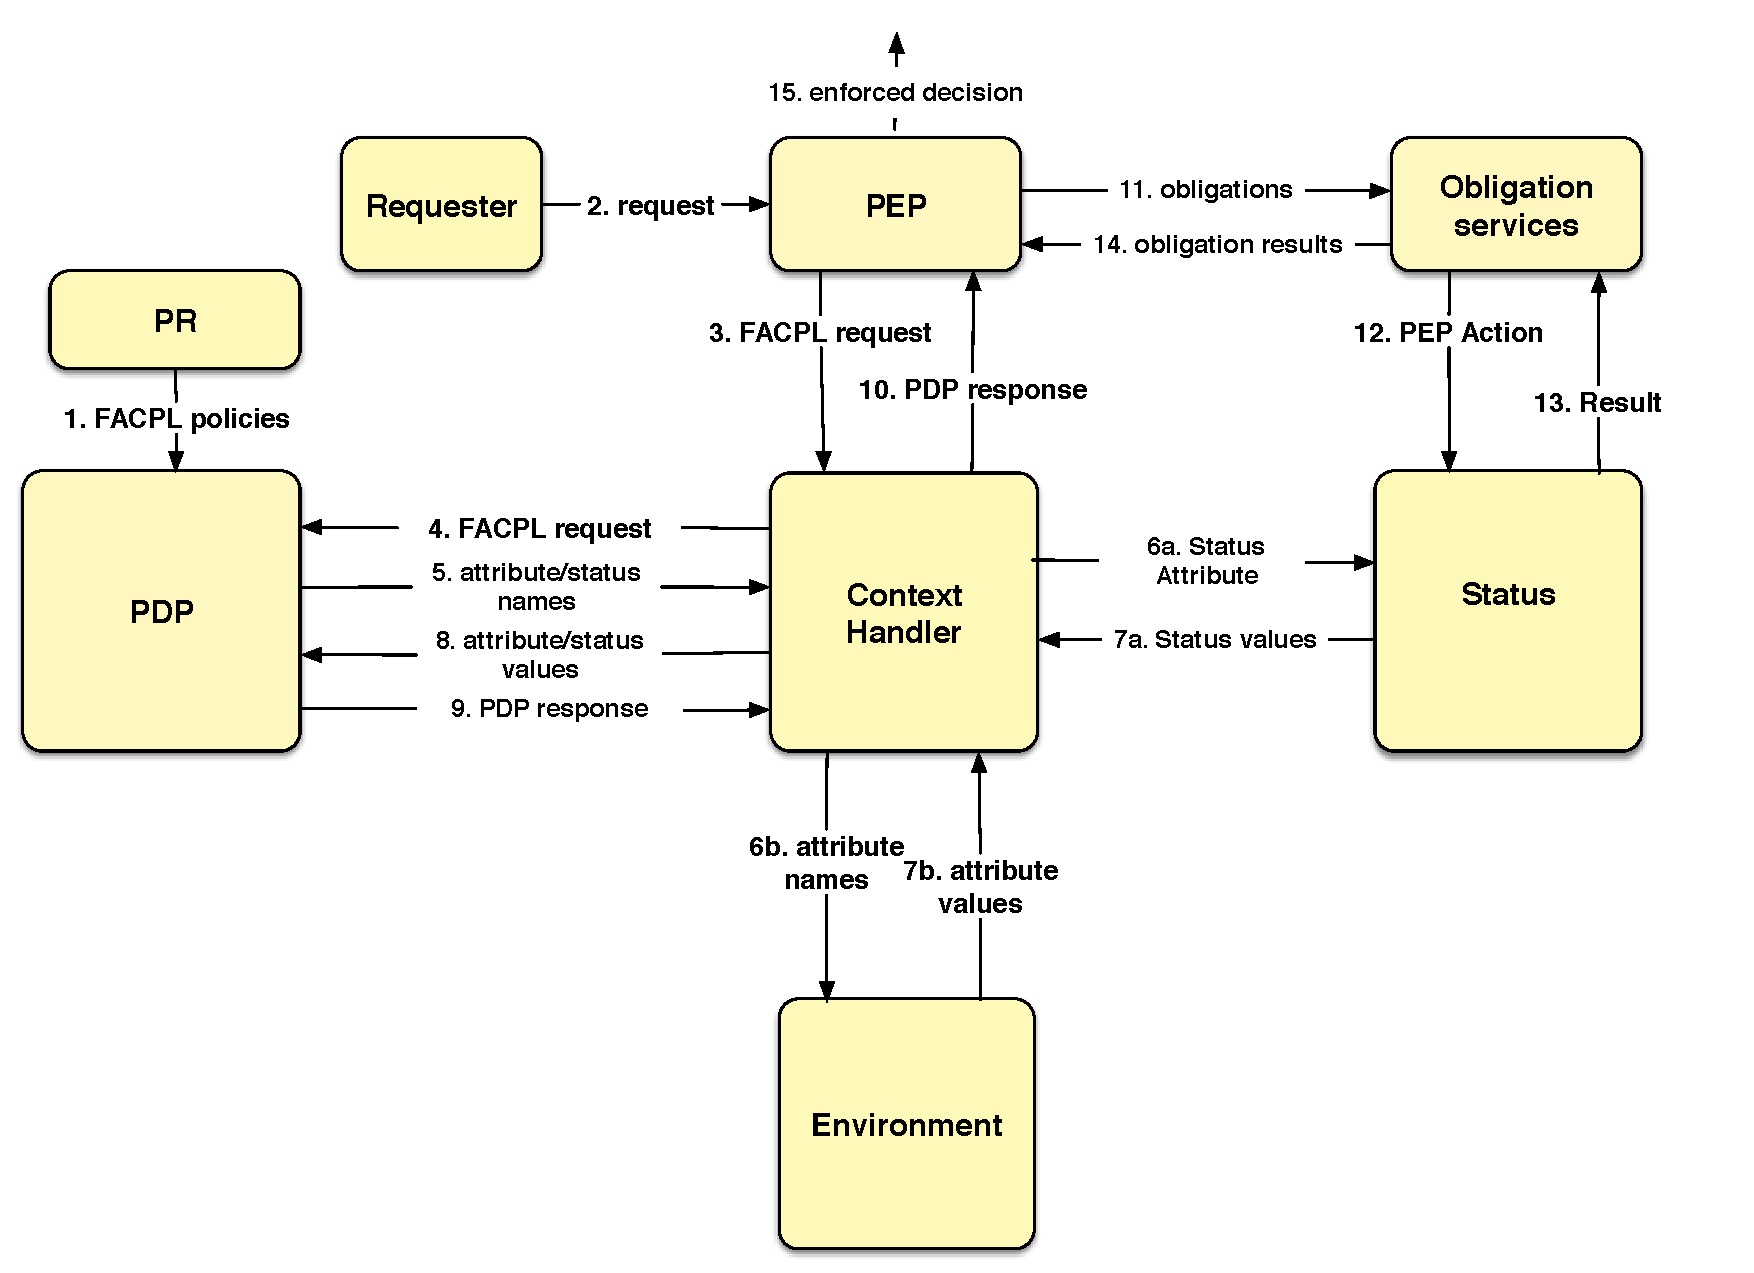
\includegraphics[scale = 0.5]{./Chapters/Image/evalvect.pdf}
 \caption{Valutazione dopo lo stato}
 \label{fig:evalStatus}
\end{figure}

Come si nota in Figura \ref{fig:evalStatus} è stato aggiunto un componente alla struttura della valutazione.
Questo componente rappresenta lo \status \ (Stato), al quale il \ac{PDP} e \ac{PEP} ci accedono tramite attributi.
Questi attributi vengono chiamati \statusattribute. \par
Analizziamo quindi, a scopo esemplificativo, come viene gestita la presenza dello stato. Inizialmente viene definito il sistema, che ora rispetto a quelli già citati in Sezione~\ref{sec:valutazione_facpl}, ha un componente in più, ovvero lo Stato.
Fino al quarto step il comportamento è analogo a quello precedente, mentre cambia negli step successivi.\\ \par
Al quinto step il \textit{PDP} non necessiterà solo dei normali attributi d'ambiente, ma necessiterà anche degli \statusattribute \ coinvolti nella richiesta effettuata. Il \textit{Context Handler} quindi non andrà solo a fare la ricerca all'interno dell'environment, ma andrà a cercare anche gli \statusattribute \ all'interno dello \status.\\ \par
A questo punto, quando il \ac{PDP} avrà tutte le informazioni necessarie si potrà passare alla vera e propria valutazione della richiesta che avviene come sempre.\\ \par
Nel caso in cui viene restituto \permit \ o \deny \ è necessario fare l'enforcement della risposta del \ac{PDP}. Questo processo differisce dal precedente poiché ora sono state implementate nuove azioni sullo stato che devono essere eseguite dal \ac{PEP} (Passo 11-14). Le nuove azioni sono eseguite attraverso un nuovo tipo di obligations, chiamate \textit{ObligationStatus}. 
Quest'ultime vengono valutate dal \ac{PEP} alla pari di una normale Obligation, ma la sostanziale differenza tra esse ed una normale Obligation è legata alla funzione che contengono. Mentre le normali Obligation conterranno generiche funzioni, come creare un log o mandare una mail, le Obligation Status potranno eseguire azioni per modificare lo stato del sistema.
Una volta effettuato l'enforcement viene restituta la decisione finale.



% section estensione_del_processo_di_valutazione (end)

\section{Estensione Linguistica} % (fold)
\label{sec:estensione_linguistica}
Per implementare queste nuove funzionalità è stata modificata anche la grammatica di \ac{FACPL}.
Nella grammatica estesa sono state aggiunte nuove regole di produzione e simboli terminali che 
codificano le nuove funzionalità.\\ \par

\begin{table}[h]
\centering
\small
\caption{Sintassi di $FACPL_{PB}$} 
$
\begin{array}{@{\,}r@{\ \ }r@{\ }r@{\ \ }l@{\ }}

&&&\\[-.2cm]
{\textbf{Policy Authorisation Systems}} &
\mathit{PAS} & ::= & ( \,  \x{pep:} \, \mathit{EnfAlg}\ \ \x{pdp:}\, \mathit{PDP} \, \  \x({status:}\, \mathit{
[Attribute]^+})^*)
\\[.2cm]
{\textbf{Attribute}} &
\mathit{Attribute}
& ::= & (\mathit{Type} \ \mathit{Identifier} \ (= Value )^{?})
\\[.2cm]
{\textbf{Type}} &
\mathit{Type}
& ::= & \x{int} \ | \ \x{boolean} \ | \ \x{date} \ | \ \x{float}
\\[.2cm]
{\textbf{Enforcement algorithms}} &
\mathit{EnfAlg}
& ::= & \based \Sep \denyBiased \Sep \permitBiased 
\\[.2cm]
{\textbf{Policy Decision Points}} &
\mathit{PDP} & ::= & \pdpPol{\algNT\ }{\x{policies:} \, \mathit{Policy}^{+}}
\\[.2cm]
{\textbf{Combining algorithms}} &
\algNT & ::= & \permitOver \Sep \denyOver \Sep \denyUnless \Sep \permitUnless \\
&& \mid &
\firstApp \Sep \onlyOneApp \Sep \weakCon \Sep \strongCon 
\\[.2cm]
\textbf{fulfilment strategies} & \delta
& ::= & 
\greedy \Sep \all 
\\[.2cm]
{\textbf{Policies}} &
\mathit{Policy} & ::= &
\ruleOpt{\mathit{Effect}\ \ \x{target:} \, Expr\ \ \x{obl:} \, \mathit{Obligation}^{*} \, } \\
&& \mid &
\{ \algNT\ \ \x{target:} \, Expr\ \ \\
&&  &
\x{policies:} \, \mathit{Policy}^{+}  \ \ \x{obl:} \, \mathit{Obligation}^{*} \, \}
\\[.2cm]
{\textbf{Effects}} &
\mathit{Effect} & ::= & \permit \Sep \deny
\\[.2cm]
{\textbf{Obligations}} &
\mathit{Obligation} & ::= & [ \, \mathit{Effect} \ \ \mathit{ObType} \ \ \obl{Expr} \, ]
\\[.2cm]
{\textbf{PepAction}} & \mathit{PepAction} & ::= & \, \x{add(\mathit{Attribute}, int)} \Sep \x{flag(\mathit{Attribute}, boolean)} \\ 
&& & \Sep \x{sumDate(\mathit{Attribute}, date)} \Sep \x{div(\mathit{Attribute}, int)} \\
&& & \Sep \x{add(\mathit{Attribute}, float)} \ \Sep \x{mul(\mathit{Attribute}, float)} \\
&& & \Sep \x{mul(\mathit{Attribute}, int)} \ \Sep \x{div(\mathit{Attribute}, float)} \\
&& & \Sep \x{sub(\mathit{Attribute}, int)} \ \Sep \x{sub(\mathit{Attribute}, float)} \\
&& & \Sep \x{sumString(\mathit{Attribute}, string)} \\ 
&& & \Sep \x{setValue(\mathit{Attribute}, string)}\\
&& & \Sep \x{setDate(\mathit{Attribute}, date)}  
\\[.2cm]
{\textbf{Obligation Types}} &
\mathit{ObType} & ::= & M \Sep O
\\[.4cm]
\textbf{Expressions}&
\mathit{Expr} & ::= &
\mathit{Name} \Sep \mathit{Value}  \\
& & \mid &\x{and(\mathit{Expr}, \mathit{Expr})} \Sep \x{or(\mathit{Expr}, \mathit{Expr})} \Sep \x{not(\mathit{Expr})} \\
& & \mid &
 \x{equal(\mathit{Expr},\mathit{Expr})}  \Sep \x{in}(\mathit{Expr}, \mathit{Expr}) \\
& & \mid & \x{greater}\textrm{-}\x{than(\mathit{Expr},\mathit{Expr})} \Sep \x{add(\mathit{Expr} ,\mathit{Expr} )}\\ 
& & \mid & \x{subtract(\mathit{Expr} ,\mathit{Expr} )} \Sep \x{divide(\mathit{Expr} ,\mathit{Expr} )}\\
& & \mid & \x{multiply(\mathit{Expr} ,\mathit{Expr} )}  \Sep \x{less}\textrm{-}\x{than(\mathit{Expr}, \mathit{Expr})}\\
\\[.2cm]
%
\textbf{Attribute Names} & 
\mathit{Name} & ::= & \mathit{Identifier}/\mathit{Identifier} \ | \ \mathit{Status}/\mathit{Identifier}\\[.2cm]
%
\textbf{Literal Values} &
\mathit{Value} & ::= & \x{true} \mid \x{false} \mid \mathit{Double} \mid \mathit{String} \mid \mathit{Date}
\\[.4cm]
{\textbf{Requests}} &
\mathit{Request} & ::= & {\attribute{\mathit{Name}}{\mathit{Value}}}^{+}
\\[.1cm]
\end{array}
$
\label{tab:facpl_new_syntax}
\end{table}




Come è facilmente osservabile dalla consultazione della Tabella~\ref{tab:facpl_new_syntax} le aggiunte rispetto alla tabella riporta in Sezione~\ref{sec:facpl_syntax} sono state diverse, vediamo adesso quali sono.\\ \par
La prima modifica è nel \ac{PAS}, cioè  lo \status, che è della forma $$status: Attribute$$ ed è formato da uno o più \textit{Attribute}.\\ \par
Passiamo ora a descrivere \textit{Attribute} che è della forma $$(Type\ Identifier (= Value)^?)$$
questo tipo particolare di attribute, che è lo \statusattribute \ descritto in precedenza, è formato innanzitutto da un \textit{Type}, dopo il tipo è richiesta una generica stringa chiamata \textit{Identifier}, che sarà un generico nome da dare all'attributo, infine viene richiesto un \textit{Value}, ovvero un valore, che in questo caso è opzionale, all'atto pratico vuol dire che l'attributo di stato potrà essere inizializzato con un valore oppure potrà essere solamente definito, lasciando che il valore sia quello di default.

\textit{Type} è il tipo che avrà l'attributo di stato, e potrà essere \texttt{int, boolean, date o double}.\\ \par
La regola \textit{PepAction} è stata modificata in modo tale che includesse nuove funzioni per operare sugli attributi di stato.
Infine l'ultima regola di produzione modificata è stata quella riguardante \textit{Attribute Names}, in questo caso è stata semplicemente aggiunto, a fianco di \textit{Identifier/Identifier}, una nuova produzione Status/\textit{Identifier}. Questa nuova produzione serve semplicemente per permettere il confronto tra attributi di stato attraverso le già esistenti \textit{Expression}.
La sintassi delle risposte è rimasta invariata.

% section estensione_linguistica (end)

\section{Semantica} % (fold)
\label{sec:semantica}
La semantica di FACPL rimane molto simile a quella descritta in Sezione \ref{sec:semantica_originale}, quindi verranno di seguito descritte in modo informale solo le novità introdotte.\\ \par
La prima di queste riguarda la valutazione delle richieste dal \ac{PDP}. Il \ac{PDP} ora non si deve più basare solo su richieste totalmente scollegate l'una dall'altra, e quindi è stato introdotto il concetto di \status.
Lo stato permette di rappresentare il comportamento passato del sistema, e lo fa introducendo una nuova serie di attributi chiamati \statusattribute.\\ \par
Nel linguaggio questo nuovo tipo di attributi viene considerato al pari di normali attributi, quindi si ha la possibilità di effettuare tutte le operazioni di confronto tra di essi, ma in più si deve avere la possibilità di modificarli e memorizzarli in modo da poterli sfruttare per \textit{Usage Control}.\\ \par

Per questo sono state aggiunte delle \textit{Pep Action}, ovvero delle azioni eseguite dal \ac{PEP} in seguito alla valutazione di \textit{Obligations status}. La prima di queste è l'addizione, 
 e permette, in seguito alla valutazione di una \textit{Obligations}, l'aggiunta di un valore numerico, definito dallo sviluppatore, ad uno \statusattribute \ di tipo \texttt{double} o \texttt{int}. 
\begin{verbatim}
 obl:
     [permit M add(counter, 2)]
\end{verbatim}
Per esempio l'esecuzione di questa \textit{Obligation} su un'attributo, chiamato \textit{counter}, inizializzato a $0$, porterà l'attributo al 
valore 2. 

L'operazione di somma è stata implementata anche per altri due tipi, \texttt{Date} e \texttt{String}.
Oltre all'addizione sono presenti funzioni per la sottrazione, divisione e moltiplicazione che operano in modo analogo a questa appena descritta, ma sono definite soltanto su tipi numerici.

Un'altra operazione implementata modifica il valore originale di uno \statusattribute \ con il valore passatogli come secondo parametro.
\begin{verbatim}
 obl:
     [permit M flag(isFoo, true)]
\end{verbatim}
L'esecuzione con successo di questa \textit{Obligation} porterà l'attributo \textit{flag} ad avere un valore \texttt{true}. Questo tipo di operazione è stata definita anche per il tipo \texttt{Date} e \texttt{String}.

Vediamo ora un esempio di questa nuova estensione, prenderemo spunto dal primo caso trattato in precedenza nella Sezione~\ref{sec:estensione_del_processo_di_valutazione}.
%SOSTITUIRE CON LISTINGS PER FACPL
\lstinputlisting[language = FACPL, caption = {Esempio per la sintassi}\label{lst:esempio_sintassi}]{./Source/first_example_facpl}
In questo esempio (Codice \ref{lst:esempio_sintassi}) si può vedere come nel PAS è stato definito uno stato, con al suo interno uno solo attributo inizializzato con valore $0$.
Successivamente si può notare nella \textit{Rule} che viene fatto un controllo sul valore di quest'attributo.
Infine nella \textit{Obligation} si può notare come viene aggiornato lo stato dell'attributo in base al risultato della valutazione della \textit{Rule}.

\section{Formalizzazione dei case study} % (fold)
\label{sec:esempi}

Queste nuove funzionalità introdotte servono allo scopo descritto in Sezione~\ref{sec:usage_control}, ovvero l'implementazione di un nuovo modello chiamato \textit{Usage Control}.
In questi due semplici case study lo stato gioca un ruolo fondamentale, in quanto il sistema di access control, per poter soddisfare requisiti di consistenza deve tener traccia del comportamento passato.
Mostreremo ora l'implementazione in \ac{FACPL} dei due esempi trattati in Sezione~\ref{sec:usage_control}. Per comodità è usata la sintassi del plugin di Eclipse, che differisce leggermente da quella presentata in \ref{sec:estensione_linguistica}. 

\subsection{Accesso ai file} % (fold)
\label{ssub:primo_esempio}
Il primo esempio in Sezione~\ref{sec:usage_control} poneva una regola sull'accesso ai file, ovvero permetteva un massimo di due persone in contemporanea che potevano effettuare l'accesso in lettura oppure un massimo di una persona che poteva ottenere l'accesso in scrittura. \par
Tutte le policy che saranno mostrate in questa sezione sono incluse in un \textit{PolicySet} che racchiude al suo interno un espressione di tipo target, mostrata in Codice~\ref{lst:PrimoEsempio_FACPL_target}.
\lstinputlisting[language = FACPL, linerange = 1-2,  caption = {Target PolicySet}\label{lst:PrimoEsempio_FACPL_target}]{./Source/EsempioReadWrite_facpl.fpl}
Il target del PolicySet \texttt{ReadWrite\_Policy} verifica che le richieste provengano da utenti che hanno nome \textit{Alice} o \textit{Bob}, in caso contrario il responso sarà \texttt{Not Applicable}. \par
Successivamente sono state scritte quattro policy per gestire le quattro operazioni possibili, ovvero \texttt{read}, \texttt{write}, \texttt{stopRead} ed infine \texttt{stopWrite}. \par
Prendiamo in considerazione la policy mostrata in Codice~\ref{lst:PrimoEsempio_FACPL_write}, ovvero quella per la \texttt{write}. Come prima è presente un target, che richiede questa volta due diverse condizioni, la prima riguarda l'id del file richiesto, la seconda invece richiede che l'azione sia \texttt{write}. Le parti interessanti di questa policy sono due, la prima riguarda la \textit{Rule}, la seconda la \textit{Obligation}. \par
La \textit{Rule} restituisce \texttt{permit} se le due condizioni dell'equal sono vere, come si può facilmente notare l'operazione di confronto non viene fatta tra una stringa ed un normale attributo, ma tra una stringa ed uno \statusattribute. \par
L'ultima cosa da notare è l'unica \textit{Obligation} presente per questa policy. Questo tipo particolare di \textit{Obligation}, ha sempre al suo interno un'azione che verrà eseguita dal PEP, questa volta però non sarà una semplice azione come scrivere un log o mandare una mail, l'azione andrà a modificare lo stato del sistema, mettendo il valore \texttt{true} all'attributo \textit{isWriting}.
\lstinputlisting[language = FACPL, linerange = 4-13, firstnumber = 4, caption = {Policy Write}\label{lst:PrimoEsempio_FACPL_write}]{./Source/EsempioReadWrite_facpl.fpl}
Successivamente si prende in considerazione la policy per l'operazione \texttt{stopWrite}, mostrata in Codice~\ref{lst:PrimoEsempio_FACPL_stopwrite}.
\lstinputlisting[language = FACPL, linerange = 24-32, firstnumber = 24, caption = {Policy StopWrite}\label{lst:PrimoEsempio_FACPL_stopwrite}]{./Source/EsempioReadWrite_facpl.fpl}
Il target definito da questa policy è molto simile a quello precedente, la differenza è nella seconda parte: in questo caso l'azione richiesta non è \texttt{Write}, ma \texttt{StopWrite}.\par
Come prima c'è una \textit{Rule} all'interno che esegue un confronto tra uno \statusattribute\ ed un valore, in questo caso \texttt{true}. Questo confronto in questo caso serve per verificare la reale presenza di uno scrittore al momento della richiesta. 
Nel caso fosse presente, e quindi la regola restituisse \texttt{true}, viene eseguita la Obligation Status che si occupa della modifica dello stato.
Le altre policy, per definire le restanti due operazioni, sono analoghe a quelle appena descritte e si possono trovare in Codice~\ref{lst:PrimoEsempio_FACPL}.
\subsubsection{Valutazione}
Prendiamo ora una serie di richieste ed analizziamone la loro valutazione.
\lstinputlisting[language = FACPL, caption = {Richieste del primo esempio}\label{lst:PrimoEsempioRichieste_FACPL}]{./Source/EsempioReadWrite_facpl_richieste.fpl}
La prima richiesta proviene da Alice, e sarà una lettura sul file1, la successiva proviene da Bob, è sempre sul file1, ma l'azione richiesta è di scrittura. Le altre sono analoghe.\par

L'output di queste richieste è mostrato in Tabella~\ref{tab:risultati_1}. Analizziamo ora il motivo di queste decisioni. Nella prima richiesta ovviamente nessuno sta leggendo o scrivendo, quindi viene tranquillamente restituito \permit. Visto che è presente una \textit{obligation} lo stato verrà aggiornato, sommando un'unità al contatore di letture.
Alla seconda richiesta l'utente richiede la scrittura, che gli viene negata perché c'è già qualcuno che sta leggendo, però lo stesso utente effettua un'altra richiesta, questa volta in lettura, che gli viene concessa.\\ \par
La quarta e la quinta richiesta vengono fatte per avvisare il sistema che la lettura è terminata, ovviamente la risposta è \permit, e la \textit{obligation} corrispondente decrementerà il contatore.
La sesta ed ultima richiesta è una scrittura, che questa volta viene permessa, poiché nessuno sta scrivendo o leggendo.
\begin{table}[H]
\centering
\footnotesize
\caption{Risultati della valutazione}
\label{tab:risultati_1}
\begin{tabular}{cccc}
\multicolumn{1}{l}{} & \textbf{Risultato} & \textbf{Stato Prima} & \textbf{Stato dopo} \\ \hline
\textbf{Richiesta 1} & \textit{PERMIT} & \begin{tabular}[c]{@{}c@{}}isWriting = false\\ CounterReadFile1 = 0\end{tabular} & \begin{tabular}[c]{@{}c@{}}isWriting = false\\ CounterReadFile1 = 1\end{tabular} \\ \hline
\textbf{Richiesta 2} & \textit{DENY} & \begin{tabular}[c]{@{}c@{}}isWriting = false\\ CounterReadFile1 = 1\end{tabular} & \begin{tabular}[c]{@{}c@{}}isWriting = false\\ CounterReadFile1 = 1\end{tabular} \\ \hline
\textbf{Richiesta 3} & \textit{PERMIT} & \begin{tabular}[c]{@{}c@{}}isWriting = false\\ CounterReadFile1 = 1\end{tabular} & \begin{tabular}[c]{@{}c@{}}isWriting = false\\ CounterReadFile1 = 2\end{tabular} \\ \hline
\textbf{Richiesta 4} & \textit{PERMIT} & \begin{tabular}[c]{@{}c@{}}isWriting = false\\ CounterReadFile1 = 2\end{tabular} & \begin{tabular}[c]{@{}c@{}}isWriting = false\\ CounterReadFile1 = 1\end{tabular} \\ \hline
\textbf{Richiesta 5} & \textit{PERMIT} & \begin{tabular}[c]{@{}c@{}}isWriting = false\\ CounterReadFile1 = 1\end{tabular} & \begin{tabular}[c]{@{}c@{}}isWriting = false\\ CounterReadFile1 = 0\end{tabular} \\ \hline
\textbf{Richiesta 6} & \textit{PERMIT} & \begin{tabular}[c]{@{}c@{}}isWriting = false\\ CounterReadFile1 = 0\end{tabular} & \begin{tabular}[c]{@{}c@{}}isWriting = true\\ CounterReadFile1 = 0\end{tabular} \\ \hline
\end{tabular}
\end{table}



\subsection{Noleggio e acquisto di contenuti} % (fold)
\label{sub:secondo_esempio}

In questo secondo esempio analizzeremo il caso di un'azienda di distribuzione di contenuti multimediali che vuole regolare l'accesso di quest'ultimi attraverso policy.
Faremo un breve esempio con un solo file e due utenti, uno dei due utenti comprerà il file, l'altro lo noleggierà a tempo determinato.
Nel codice~\ref{lst:SecondoEsempio_FACPL} vengono mostrate solo una parte delle policy presenti nel Codice completo ~\ref{lst:SecEsCompl} \ mostrato in Appendice~\ref{cap:appendiceA}.
\lstinputlisting[firstline = 1, lastline = 39, language = FACPL, caption = {Secondo Esempio}\label{lst:SecondoEsempio_FACPL}]{./Source/second_example_facpl}
Queste due policy, e anche le altre che non sono state mostrate, sono racchiuse tutte all'interno del \textit{Policy Set} Negozio il quale come prima cosa verifica se chi ha fatto la richiesta ha un determinato nome, in questo caso \textit{Bob} o \textit{Alice}.\\ \par
Successivamente, se uno dei due effettua la richiesta di \texttt{BUY}, ovvero l'acquisto senza alcun tipo di limitazione, si entra nella prima policy e, tramite le \textit{Obligation} si cambia l'attributo di stato. Invece se un utente decidesse di effettuare il noleggio con la modalità dove si limita il numero di visioni si entrerebbe nella seconda \textit{Policy Set} la quale, attraverso \textit{Obligations} aumenterà il numero di visioni di due unità. Analogo è il caso del noleggio a tempo.\\ \par
Per disciplinare la visione è presente un altro \textit{Policy Set}, mostrato anch'esso parzialmente in codice~\ref{lst:secondo_esempio_view}.
\lstinputlisting[firstline = 59, lastline = 71, language = FACPL, caption = {Secondo Esempio}\label{lst:secondo_esempio_view}]{./Source/second_example_facpl}
\subsubsection{Valutazione}
Mostriamo ora in Codice~\ref{lst:richieste_2} alcune richieste che possono essere fatte al sistema ed analizziamo le risposte che produrranno, in Tabella~\ref{tab:valutazione_2} è mostrato un quadro riassuntivo del risultato delle richieste.
\lstinputlisting[language = FACPL, caption = {Richieste del Secondo Esempio}\label{lst:richieste_2}]{./Source/second_example_request}
La prima e la seconda richiesta sono richieste di visione, che ovviamente restituiranno entrambe \deny, in quanto lo stato del sistema non è stato modificato da nessuno poiché nè Alice nè Bob hanno effettuato acquisti o noleggi.
Successivamente Alice effettuerà un acquisto, e quindi tramite la Obligation Status verrà modificato lo stato del sistema, accreditando così l'acquisto. Dopo aver effettuato questa richiesta Alice ne effettua un'altra, questa volta di visione. 
A questo punto la policy che disciplina quest'ultima richiesta di Alice effettua una verifica dello \statusattribute \ \textit{AccessTypeAlice}, e visto che lo trova cambiato dalla precedente richiesta di acquisto permette la visione.
Bob, a cui all'inizio era stata negata la visione effettuerà una richiesta di noleggio e quindi cambierà lo stato. Dopo, sempre Bob, richiede la visione, il risultato di entrambe sarà ovviamente \permit.
% subsection secondo_esempio (end)

\begin{table}[H]
\centering
\footnotesize
\caption{Riassunto Valutazione}
\label{tab:valutazione_2}
\begin{tabular}{cccc}
\multicolumn{1}{l}{} & \textbf{Risultato} & \textbf{Stato Prima} & \textbf{Stato dopo} \\ \hline
\textbf{Richiesta 1} & \textit{DENY} & \begin{tabular}[c]{@{}c@{}}AccessTypeAlice = null\\ AccessTypeBob = null\end{tabular} & \begin{tabular}[c]{@{}c@{}}AccessTypeAlice = null\\ AccessTypeBob = null\end{tabular} \\ \hline
\textbf{Richiesta 2} & \textit{DENY} & \begin{tabular}[c]{@{}c@{}}AccessTypeAlice = null\\ AccessTypeBob = null\end{tabular} & \begin{tabular}[c]{@{}c@{}}AccessTypeAlice = null\\ AccessTypeBob = null\end{tabular} \\ \hline
\textbf{Richiesta 3} & \textit{PERMIT} & \begin{tabular}[c]{@{}c@{}}AccessTypeAlice = null\\ AccessTypeBob = null\end{tabular} & \begin{tabular}[c]{@{}c@{}}AccessTypeAlice = BUY\\ AccessTypeBob = null\end{tabular} \\ \hline
\textbf{Richiesta 4} & \textit{PERMIT} & \begin{tabular}[c]{@{}c@{}}AccessTypeAlice = BUY\\ AccessTypeBob = null\end{tabular} & \begin{tabular}[c]{@{}c@{}}AccessTypeAlice = BUY\\ AccessTypeBob = null\end{tabular} \\ \hline
\textbf{Richiesta 5} & \textit{PERMIT} & \begin{tabular}[c]{@{}c@{}}AccessTypeAlice = BUY\\ AccessTypeBob = null\end{tabular} & \begin{tabular}[c]{@{}c@{}}AccessTypeAlice = BUY\\ AccessTypeBob = TIME\\ BobFile1Expiration = 2016/04/22\end{tabular} \\ \hline
\textbf{Richiesta 6} & \textit{PERMIT} & \begin{tabular}[c]{@{}c@{}}AccessTypeAlice = BUY\\ AccessTypeBob = TIME\\ BobFile1Expiration = 2016/04/22\end{tabular} & \begin{tabular}[c]{@{}c@{}}AccessTypeAlice = BUY\\ AccessTypeBob = TIME\\ BobFile1Expiration = 2016/04/22\end{tabular} \\ \hline
\end{tabular}
\end{table}


% section esempi (end)
